\documentclass[BTech]{iitpdiss}
\usepackage{times}
 \usepackage{t1enc}
\usepackage{url}
\usepackage{color}
\usepackage{graphicx} % for including graphics files
\usepackage{ifpdf} % to use same .tex file for both latex & pdflatex the following specifies different options to hyperref depending on whether latex or pdflatex is being run.
\ifpdf
\usepackage[colorlinks=,linkcolor=blue,urlcolor=blue,citecolor=blue,plainpages=false,pdfpagelabels,breaklinks]{hyperref}
\else
\usepackage[colorlinks,linkcolor=blue,urlcolor=blue,citecolor=blue,plainpages=false,pdfpagelabels,linktocpage]{hyperref}
\fi
\usepackage{epstopdf}
\usepackage{hyperref} % hyperlinks for references.
\usepackage{amsmath,amssymb} % easier math formulae, align, subequations \ldots

\begin{document}

%%%%%%%%%%%%%%%%%%%%%%%%%%%%%%%%%%%%%%%%%%%%%%%%%%%%%%%%%%%%%%%%%%%%%%
% Title page

\title{OPTIMAL CHARGING OF HYBRID ELECTRIC VEHICLE IN SMART GRID ENVIRONMENT}

\author{Venkatesh Chaturwedi}
\rollno{1101EE37}
\date{SEPTEMBER 2014}
\department{ELECTRICAL ENGINEERING}

%\nocite{*}
\maketitle

%%%%%%%%%%%%%%%%%%%%%%%%%%%%%%%%%%%%%%%%%%%%%%%%%%%%%%%%%%%%%%%%%%%%%%
% Certificate
\certificate

\vspace*{0.5in}

\noindent This is to certify that the thesis titled {\bf OPTIMAL CHARGING OF HYBRID ELECTRIC VEHICLE IN SMART GRID ENVIRONMENT}, submitted by {\bf Venkatesh Chaturwedi },
to the Indian Institute of Technology, Patna, for
the award of the degree of {\bf Bachelor of Technology}, is a bona fide
record of the research work done by him under our supervision.  The
contents of this thesis, in full or in parts, have not been submitted
to any other Institute or University for the award of any degree or
diploma.

\vspace*{1.5in}

\begin{singlespacing}
	\hspace*{-0.25in}
	%\parbox{2.5in}{
	%\noindent {\bf Dr.~} \\
	%\noindent Research Guide \\ 
	%\noindent Assistant Professor \\
	%\noindent Dept. of Electrical Engineering\\
	%\noindent IIT-Patna, 800 013 \\
	%} 
	\hfill
	\parbox{2.5in}{
		\noindent {\bf Dr. S. Sivasubramani } \\
		\noindent Supervisor \\
		\noindent Assistant Professor \\
		\noindent Dept.  of  Electrical Engineering\\
		\noindent IIT-Patna, 800 013 \\
	}
\end{singlespacing}
\vspace*{0.25in}
\\
\noindent Place: Patna\\
\noindent Date: 17th September 2014


%%%%%%%%%%%%%%%%%%%%%%%%%%%%%%%%%%%%%%%%%%%%%%%%%%%%%%%%%%%%%%%%%%%%%%
% Acknowledgements
\acknowledgements

Thanks to all those who made \TeX\ and \LaTeX\ what it is today.

%%%%%%%%%%%%%%%%%%%%%%%%%%%%%%%%%%%%%%%%%%%%%%%%%%%%%%%%%%%%%%%%%%%%%%
% Abstract

\abstract

\noindent KEYWORDS: \hspace*{0.5em} \parbox[t]{4.4in}{\LaTeX ; Thesis;
	Style files; Format.}

\vspace*{24pt}

\noindent A \LaTeX\ class along with a simple template thesis are
provided here.  These can be used to easily write a thesis suitable
for submission at IIT-Patna.  The class provides options to format
PhD, MS, M.Tech.\ and B.Tech.\ thesis.  It also allows one to write a
synopsis using the same class file.  Also provided is a BIB\TeX\ style
file that formats all bibliography entries as per the IITP format.

The formatting is as (as far as the author is aware) per the current
institute guidelines.

\pagebreak

%%%%%%%%%%%%%%%%%%%%%%%%%%%%%%%%%%%%%%%%%%%%%%%%%%%%%%%%%%%%%%%%%
% Table of contents etc.

\begin{singlespace}
	\tableofcontents
	\thispagestyle{empty}

	\listoftables
	\addcontentsline{toc}{chapter}{LIST OF TABLES}
	\listoffigures
	\addcontentsline{toc}{chapter}{LIST OF FIGURES}
\end{singlespace}


%%%%%%%%%%%%%%%%%%%%%%%%%%%%%%%%%%%%%%%%%%%%%%%%%%%%%%%%%%%%%%%%%%%%%%
% Abbreviations
\abbreviations

\noindent
\begin{tabbing}
	xxxxxxxxxxx \= xxxxxxxxxxxxxxxxxxxxxxxxxxxxxxxxxxxxxxxxxxxxxxxx \kill
	\textbf{IITP}   \> Indian Institute of Technology, Patna \\
	\textbf{RTFM} \> Read the Fine Manual \\
\end{tabbing}

\pagebreak

%%%%%%%%%%%%%%%%%%%%%%%%%%%%%%%%%%%%%%%%%%%%%%%%%%%%%%%%%%%%%%%%%%%%%%
% Notation

\chapter*{\centerline{NOTATION}}
\addcontentsline{toc}{chapter}{NOTATION}

\begin{singlespace}
	\begin{tabbing}
		xxxxxxxxxxx \= xxxxxxxxxxxxxxxxxxxxxxxxxxxxxxxxxxxxxxxxxxxxxxxx \kill
		\textbf{$r$}  \> Radius, $m$ \\
		\textbf{$\alpha$}  \> Angle of thesis in degrees \\
		\textbf{$\beta$}   \> Flight path in degrees \\
	\end{tabbing}
\end{singlespace}

\pagebreak
\clearpage

% The main text will follow from this point so set the page numbering
% to arabic from here on.
\pagenumbering{arabic}


%%%%%%%%%%%%%%%%%%%%%%%%%%%%%%%%%%%%%%%%%%%%%%%%%%
% Introduction.

\chapter{INTRODUCTION}
\label{chap:intro}

Ever since machine learning has been introduced into the field of computer science, it has been spearheading breakthroughs in a number of fields. It has taken the world by storm and now, many fields will simply cease to function without these techniques. Deep learning is one sub-field of machine learning which is deeply rooted in todays society. Deep learning is now part of common man's everyday life and it will remain so for the forseeable future.

As data collection and storage becomes more prominent, machine and deep learning has continued to dominate the data space, provide insights into complex data which is simply not possible with other mathematical methods. Deep learning is one of the most rapidly expanding machine learning technologies, relying on multi-layered artificial neural networks (ANNs) implemented in digital electronics to handle big data sets, integrating and analysing massive volumes of information quickly without the need for explicit instructions. These ANNs have been modified and augmented in many ways, leading many domain specific techniques, most notable one being Convolutional Neural Networks (CNNs) which is primarily used in image analysis.
\section{Artifical Neural Networks}

Artificial neural networks refers to those algorithms which are inspired by the biological neural networks that constitute animal brains. Such systems learn to perform tasks by considering examples, generally without being programmed with any task-specific rules. For example, in image recognition, they might learn to identify images that contain cats by analyzing example images that have been manually labeled as "cat" or "no cat" and using the results to identify cats in other images. They have found most use in applications difficult to express with a traditional computer algorithm using rule-based programming.

Traditionally ANNs have been described as a black box of sorts. It has a number of input variables and output variables using simple arithmetic connections, gives output from the input.

ANNs Traditionally tend to excel where the relations between inputs and outputs are non-linear. It is practically better and more efficient at classifying or identifying non-linear relationships rather that linear ones, where it might perform worse than a more statistical approach.

\begin{figure}
	\centering
	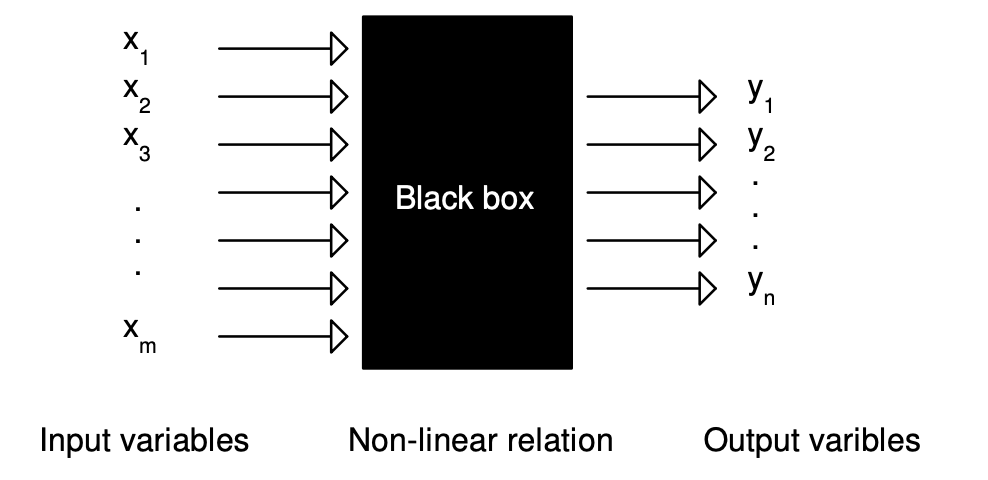
\includegraphics[width=1\textwidth]{images/ann.png}
	\caption{Schematic of a neuron}
	\label{fig:neuron}
\end{figure}

\begin{singlespace}
	\bibliographystyle{IEEEtran}
	\bibliography{refs}
\end{singlespace}


%%%%%%%%%%%%%%%%%%%%%%%%%%%%%%%%%%%%%%%%%%%%%%%%%%%%%%%%%%%%
% List of papers

%\listofpapers

%\begin{enumerate}  
%\item Authors....  \newblock
% Title...
%  \newblock {\em Journal}, Volume,
%  Page, (year).
%\end{enumerate}  
%
\end{document}
